\section{Introduction}

Small UAS carrying LiDAR, RGBD cameras, or monocular cameras using Structure from Motion (SfM) can generate 3D point clouds of nearby landing sites. Polylidar3D can transform these dense point clouds to polygonal representations of flat surfaces in real-time while accounting for obstacles. Chapter \ref{ch:landingsim} presented simulation results using Polylidar3D for real-time touchdown point selection for rooftops using on-board LiDAR and cameras. This chapter extends simulations to real-world experiments conducted at the University of Michigan Ford Motor Company Robotics Building Fly Lab. This work demonstrates the integration of multiple LiDAR scans into a larger cohesive mesh in which noise is reduced. The final mesh is then sent to Polylidar3D for polygon extraction and touchdown point selection.

We assembled a sensor package that hosts an Intel RealSense L515 LiDAR, RealSense T265 Tracking Camera, and an Odyssey x86 \acf{SBC}. Together they provide color/depth images, 6DOF tracking, and the computation power needed to implement our touchdown point selection methods presented in Chapter \ref{ch:landingsim}. Safe touchdown points are found in a cluttered indoor environment. Two separate experiments are performed: one with a hand-carried sensor package and another with the package mounted underneath a flying quadrotor.  Results indicate that our presented methods are able to identity safe touchdown points accurately and efficiently.

\section{Touchdown Point Selection}\label{sec:ch7_volume_integration}

Chapter \ref{ch:landingsim} proposed our method of selecting a touchdown point from a single scan of a rotating LiDAR sensor mounted underneath a \ac{sUAS}. The single range image is quickly transformed into a mesh of the environment.  This chapter proposes to alternatively integrate multiple scans to create a unified mesh of the environment. This integration process requires the \ac{sUAS} to have precise localization capabilities. This capability is provided by the Intel RealSense T265 tracking sensor and mounted on-board the quadrotor and validated by a motion capture system.

The L515 LiDAR is able to produce an \ac{RGBD} image by aligning  the depth and color data streams. Multiple \ac{RGBD} frames are integrated into a cohesive map using methods from Zhou et al.~\cite{zhou_dense_2013} and implemented in Open3D~\cite{zhou_open3d_2018}. The technique works by creating a truncated signed distance field within a voxel volume.  The volume is updated by deprojecting points from an RGBD image into the volume which requires both intrinsic and extrinsic parameters of the camera. The signed distance field is then extracted as a triangular mesh using the marching cubes algorithm \cite{10.1145/37401.37422}.  In this work we use a voxel size of 5cm which provides more than enough resolution for landing site decisions. At 3m of distance the range noise of the L515 LiDAR is less than 1cm \cite{nxp:tja1043}; noise is nearly removed after integrating multiple frames.

After the mesh is extracted, Polylidar3D is used to extract flat surfaces as polygons. Any obstacles embedded on the surface are captured as interior holes. The largest inscribed circle of the largest polygon is used to select a landing zone.  A circle must meet the minimum radial footprint of 0.75 meters, determined by quadrotor size, or no touchdown point is selected. We develop an open-source hardware and software platform that implements this functionality and validate it experimentally.

% and validated by a motion capture system

\section{Experimental Setup}

\subsection{Sensor Package Construction}

The sensor package is shown in Figure \ref{fig:ch7_sensor_package_pic}. The package is composed of a (1) RealSense L515 LiDAR/Color Sensor, (2) RealSense T265 Tracking Camera, (3) Odyssey x86 \ac{SBC}, and a (4) 12V Li-ion battery pack. The package is held together with 3D printed plates and standoffs having a total mass of 720 grams. The dimensions of the package are $120 \times 110 \times 50 mm$. The L515 device is mounted directly underneath the sensor package pointing down, while the T265 is mounted in the front. The Odyssey \ac{SBC} and battery are placed between the printed plates.

\begin{figure}[!htb]
  \centering
  \begin{subfigure}[t]{.40\linewidth}
    \centering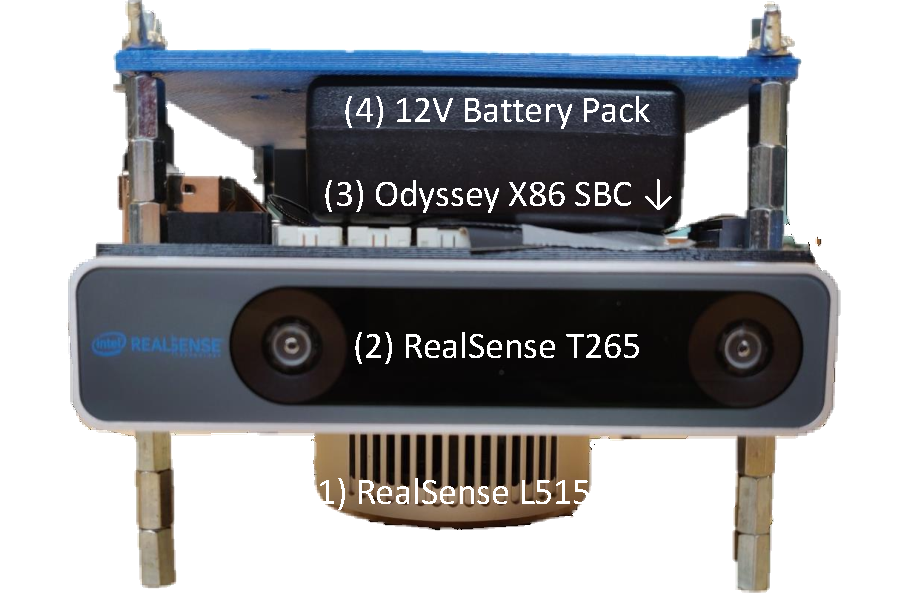
\includegraphics[page=1,clip,trim=0cm 0cm 0cm 0cm,width=.99\linewidth]{chapter_7_experiments/imgs/sensor_package.pdf}
    \caption{\label{fig:ch7_sensor_package_a}Front View}
  \end{subfigure}
  \begin{subfigure}[t]{.40\linewidth}
    \centering\includegraphics[page=3,clip,trim=0cm 0cm 0cm 0cm,width=.99\linewidth]{chapter_7_experiments/imgs/sensor_package.pdf}
    \caption{\label{fig:ch7_sensor_package_b}Underside View}
  \end{subfigure}
  \caption[Sensor package components]{Sensor package components.}\label{fig:ch7_sensor_package_pic}
\end{figure}

\subsection{Sensor Coordinate Frames}

The coordinate frames of the L515 LiDAR and T265 tracking sensors are shown in Figure \ref{fig:ch7_sensor_frames} and denoted as \{L\} and \{T\}, respectively. The L515 follows nominal camera axis conventions ($z$-axis forward, $x$-axis right) while the tracking sensor follows \acf{VR} conventions ($z$-axis backwards, $x$-axis right). The T265 outputs a 6DOF pose (position and orientation) with respect to a world frame origin denoted \{WT\} set during initialization. As a result \{WT\} follows \ac{VR} axes conventions which is non-standard in Aerospace applications. Another world frame \{WNED\} is created to be coincident to \{WT\} but rotated such that it follows NED conventions ($z$-axis down, $x$-axis forward). The reference frame of data will be indicated by a superscript, e.g., $\mathcal{P}^{L}$ denotes a point cloud in the LiDAR frame. A homogeneous transformation from frame A to frame B is denoted $\mathbf{H}^A_B$.

\begin{figure}[!htb]
  \centering
  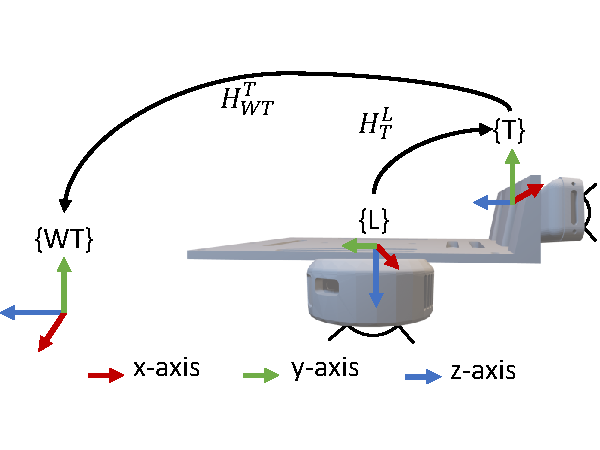
\includegraphics[page=1,clip,trim=0cm 1cm 0cm 1cm,width=.45\linewidth]{chapter_7_experiments/imgs/sensor_frames.pdf}
  \caption[Sensor package coordinate frames]{Sensor package coordinate frames.}\label{fig:ch7_sensor_frames}
\end{figure}
Volume integration as described in Section \ref{sec:ch7_volume_integration} requires LiDAR camera intrinsic and extrinsic calibration parameters. The intrinsics of the L515 are factory calibrated and provided by the RealSense SDK \cite{noauthor_github_2020-4}. The T265 pose provides the extrinsics $\mathbf{H}^{T}_{WT}$  of the T265 sensor with respect to \{WT\}. This pose must be appropriately transformed to create the extrinsics of the L515 camera in the world NED frame:
\begin{align*}
   \mathbf{H}^{L}_{WNED}  =  \mathbf{R}^{WT}_{WNED} \cdot \mathbf{H}^{T}_{WT} \cdot \mathbf{H}^{L}_{T}
\end{align*}
where $\mathbf{R}^{WT}_{WNED}$ denotes the rotation from \{WT\} to \{WNED\}. The matrix $\mathbf{H}^{L}_{WNED}$ may then transform points in \{L\} to \{WNED\} to create a mesh in this reference frame.

\subsection{Quadrotor Frame and Sensor Package Integration}

We utilize the M330 quadrotor designed at the University of Michigan Autonomous Aerospace Systems (A2Sys) Lab for all flight experiments \cite{romano_experimental_2019}. The frame measures 33cm diagonally between each pair of motors and is powered by a 4S 3000mAh LiPo battery. Markers are placed on the quadrotor frame and tracked by a \ac{MCS}. The \ac{MCS} sends pose estimates of the quadrotor to the flight controller using a wireless serial radio. The quadrotor is controlled by a custom autopilot running on a BeagleBone Blue that uses these ground truth pose estimates for position and yaw control. The sensor package is mounted directly underneath the quadrotor as shown in Figure \ref{fig:ch7_drone_frame}. The vehicle body frame \{B\} is defined by the \ac{MCS}. The total mass of the quadrotor and sensor package is 1744 grams.

\begin{figure}[!htb]
  \centering
  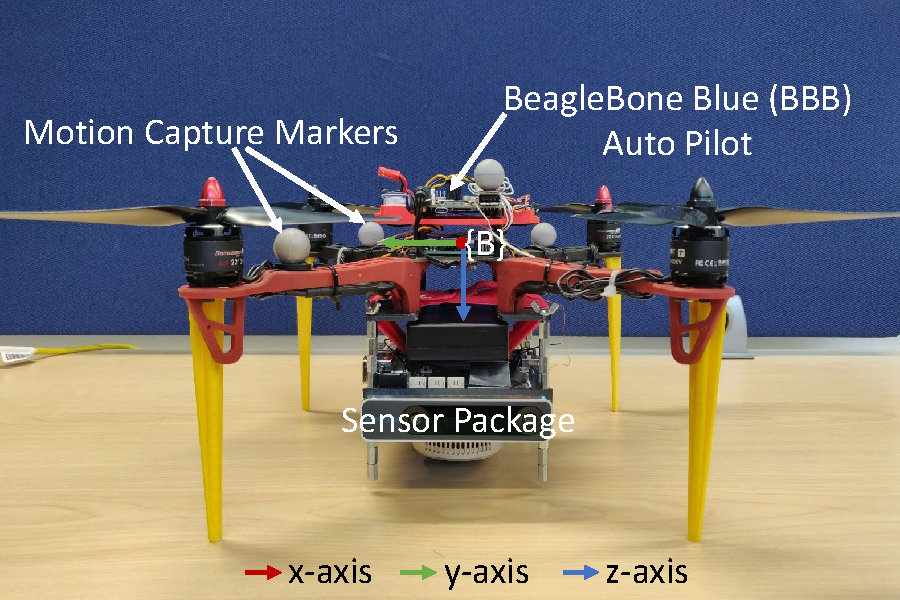
\includegraphics[page=1,clip,trim=0cm 0cm 0cm 0cm,width=.50\linewidth]{chapter_7_experiments/imgs/drone_with_sensor_package.pdf}
  \caption[Sensor package and quadrotor integration]{Sensor package quadrotor integration. The sensor package is mounted directly underneath the quadrotor. The Beagle Bone Blue autopilot, motion capture markers, and quadrotor body frame \{B\} are indicated.}\label{fig:ch7_drone_frame}
\end{figure}

We continue to use the \ac{MCS} for quadrotor position control because the T265 sensors accuracy, precision, and reliability have not been fully tested for flight experiments. The T265 is only used to generate a mesh of the environment to give a final touchdown point command to the quadrotor. Note that the T265 sensor initializes the \{WNED\} frame during startup. Therefore the quadrotor is positioned such that the \ac{MCS} coordinate frame is closely aligned with \{WNED\} before every flight. However, there is a marginal height offset ($<$ 10cm) between these frames because the T265 is mounted higher than the ground plane. All commanded touchdown points are given in the \{WNED\} frame.

\subsection{Environment}

All experiments were performed inside the University of Michigan's Ford Robotics Building Fly Lab. Four obstacles were placed on the floor including three boxes and one small ladder. The environment, obstacle labelling, and origin frame are shown in Figure \ref{fig:ch7_workspace_a}. Obstacle dimensions were measured using a ruler and placed at known positions within the environment. An overlay of the environment and obstacles is shown in Figure \ref{fig:ch7_workspace_b}. The workspace was limited to a $3.5m\times3.5m$ box centered at the \ac{MCS} origin and represents the safely navigable region for the drone also within \ac{MCS} view. Together the workspace and obstacles form a ground truth polygon to assess the accuracy of any proposed landing area created by Polylidar3D. The obstacles were chosen to have a mix of convex and non-convex shapes to challenge our polygon extraction methods. The size and placement of the obstacles were selected to prevent overloading the workspace and to provide an open area for landing. In future experiments we will diversify obstacles and their placement to further challenge our proposed methods.

\begin{figure}[!htb]
  \centering
  \begin{subfigure}[t]{.50\linewidth}
    \centering  \includegraphics[page=2,clip,trim=0cm 1cm 0cm 0cm,width=.99\linewidth]{chapter_7_experiments/imgs/ExperimentSetup.pdf}
    \caption{\label{fig:ch7_workspace_a}}
  \end{subfigure}
  \begin{subfigure}[t]{.35\linewidth}
    \centering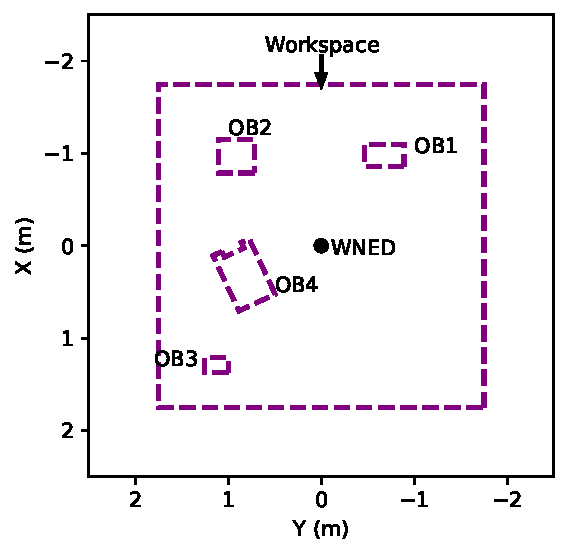
\includegraphics[page=1,clip,trim=0cm 0cm 0cm 0cm,width=.99\linewidth]{chapter_7_experiments/imgs/workspace_plot.pdf}
    \caption{\label{fig:ch7_workspace_b}}
  \end{subfigure}
  \caption[Flight lab setup]{Flight lab setup. (\subref{fig:ch7_workspace_a}) Photo of flight lab and obstacle placement. (\subref{fig:ch7_workspace_b}) Ground truth graph of the environment.}\label{fig:ch7_workspace}
\end{figure}

\subsection{Hardware and Software Integration}\label{sec:ch7_software}

The data streams and frequencies for each sensor are shown in Table \ref{table:ch7_datastreams}. Because of the real-time computational demand of integrating RGBD frames into a volume the frequency of the L515 was reduced to 6Hz. However, the authors noticed no degradation in mesh quality in comparison to running at full speed (30Hz) on a desktop computer. The resolution of the depth stream and RGB stream were set at the recommended levels from Intel to further reduce computational demand. 


\begin{table}[ht]
\centering
\caption[Sensor package details]{Sensor package details}
\label{table:ch7_datastreams}
\begin{tabular}{@{}llll@{}}
\hline\noalign{\smallskip}
Sensor                                       & Stream & Frequency  & Description                             \\ 
\noalign{\smallskip}\hline\noalign{\smallskip}
\multirow{2}{*}{L515 LiDAR Camera}           & Depth    & 6 Hz & 640X480, Depth Stream      \\
                                             & Color    & 6 Hz    & 1280X720, RGB Stream                      \\
\multirow{1}{*}{T265 Tracking Camera}         & 6DOF    & 100 Hz & Position and Orientation                         \\
\noalign{\smallskip}\hline\noalign{\smallskip}
\end{tabular}
\end{table}


Figure \ref{fig:ch7_software} shows a diagram of the devices and software used in the experiments. The top left of the diagram displays the hardware interfaces, the top right is a legend, and the bottom is the software architecture. The Odyssey \ac{SBC} communicates to the quadrotor Beaglebone Blue flight controller through a serial connection. The communication is one-way and allows the emergency landing software to command a landing position. Currently the command is issued only once, cannot be cancelled, and the quadrotor will immediately fly a constant altitude path to the position and then land. More sophisticated emergency landing logic is beyond the scope of this work.

The urgent landing software is composed of four main programs: \texttt{RS-Pub}, \texttt{RS-Integrate}, \texttt{Landing Sever}, and \texttt{Record}. Programs communicate with each other with messages using \ac{ECAL}, a fast publish-subscribe middleware that manages inter-process communication \cite{Continental_Github_ecal}. The program \texttt{RS-Pub} is responsible for configuring and gathering data from the RealSense devices and publishes shared memory messages containing \ac{RGBD} frames with pose information. The program \texttt{RS-Integrate} subscribes to these messages and will integrate them into a cohesive voxel volume using Open3D \cite{zhou_open3d_2018}. It also runs a TCP/IP server that upon request will extract a mesh from the volume. The program \texttt{Landing-Sever} contains the algorithms and software previously presented in this dissertation. This contains our own software including mesh smoothing, polygon extraction, polygon filtering, and touchdown point selection. This program also runs an interactive terminal user interface, shown in Figure \ref{fig:ch7_tui}, which allows a user to activate the emergency landing protocols. Finally, the program \texttt{Record} efficiently records all messages with synchronized timestamps. All code for this work is open-source and freely available \cite{Castagno_Github_realsensepackage}.

\begin{figure}[!tb]
    \centering  
    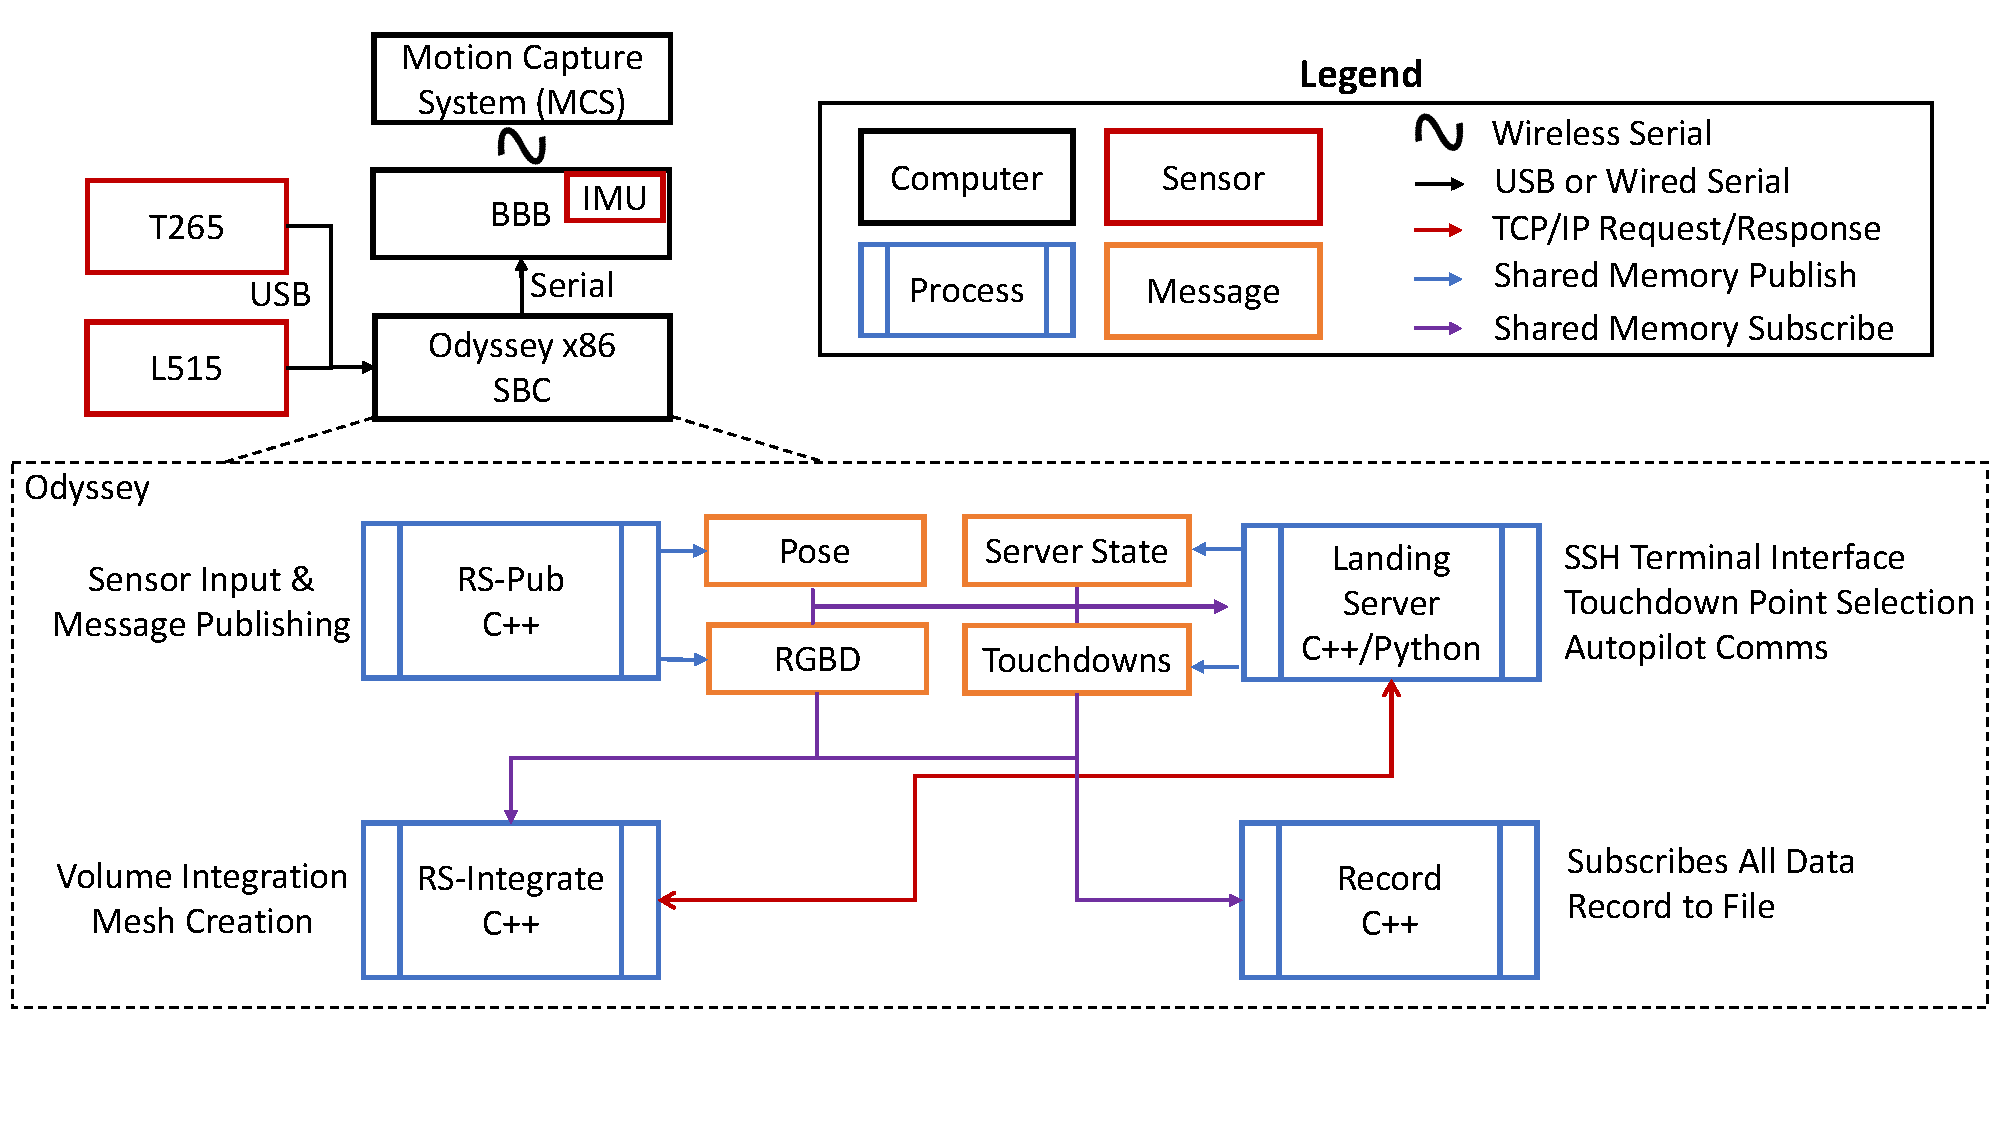
\includegraphics[page=1,clip,trim=0cm 0cm 0cm 0cm,width=.90\linewidth]{chapter_7_experiments/imgs/SoftwareOverview-v2.pdf}
    \caption[Overview of hardware interfaces and software architecture]{Overview of hardware interfaces and software architecture.}\label{fig:ch7_software}
\end{figure}

\begin{figure}[!tb]
    \centering  
    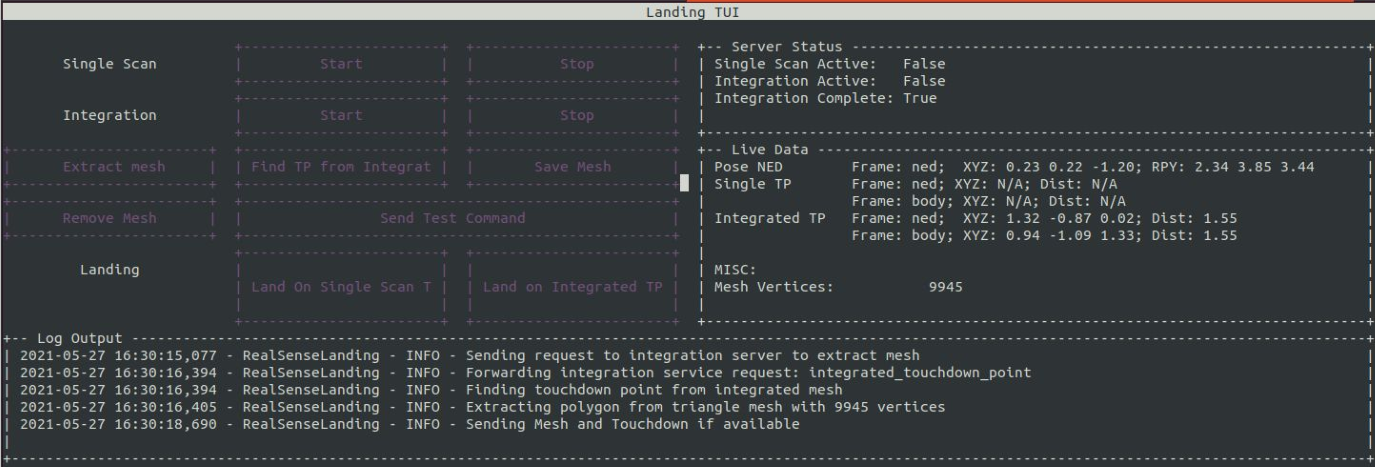
\includegraphics[page=1,clip,trim=0cm 0cm 0cm 0cm,width=.95\linewidth]{chapter_7_experiments/imgs/SensorPackage_TUI.pdf}
    \caption[Picture of terminal user interface for urgent landing]{Picture of terminal user interface for urgent landing.}\label{fig:ch7_tui}
\end{figure}

\section{Experimental Results for Touchdown Point Selection}

Sections \ref{sec:ch7_results_handcarry} and \ref{sec:ch7_results_flight} present results for hand-carry and flight tests for our touchdown point selection algorithm, respectively. Section \ref{sec:ch7_results_execution_time} provides execution timings statistics for our algorithms.  Section \ref{sec:ch7_results_t265_accuracy} presents a trajectory evaluation error analysis for the Intel T265 sensor.

\subsection{Hand Carry Test} \label{sec:ch7_results_handcarry}
\begin{figure}[!htb]
  \centering
  \begin{subfigure}[t]{.30\linewidth}
    \centering  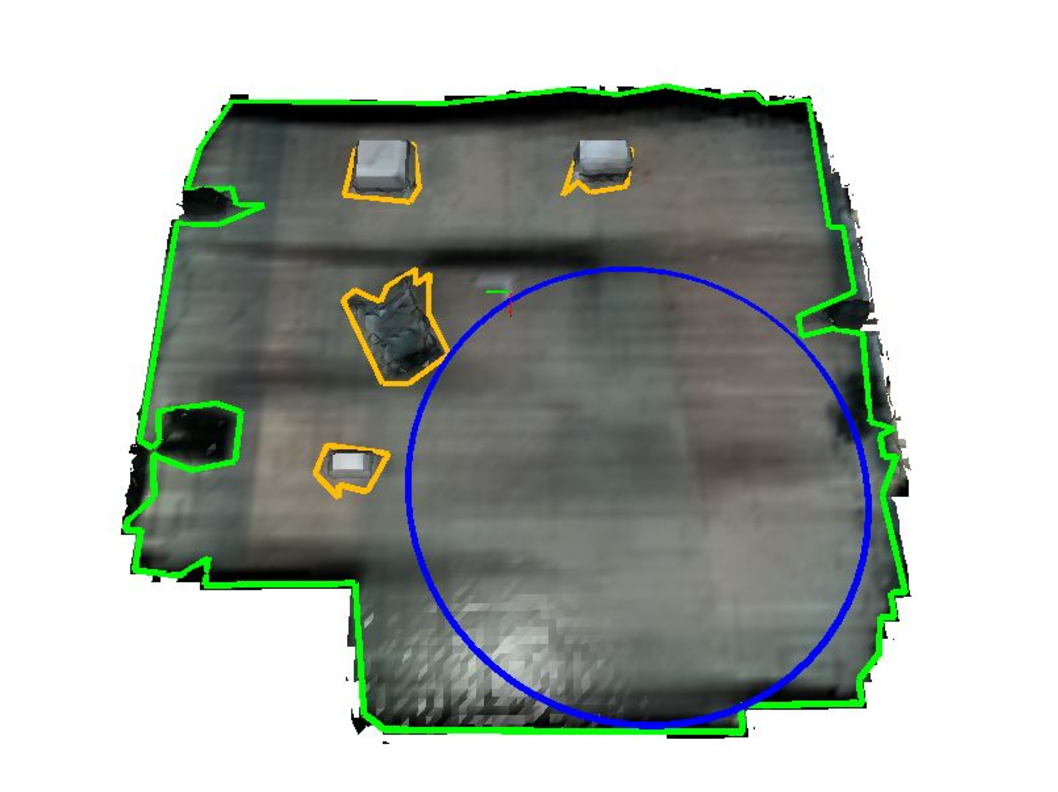
\includegraphics[page=1,clip,trim=2cm 0cm 2cm 0cm,width=.99\linewidth]{chapter_7_experiments/imgs/mesh_man_all.pdf}
    \caption{\label{fig:ch7_mesh_a}}
  \end{subfigure}
  \begin{subfigure}[t]{.30\linewidth}
    \centering  \includegraphics[page=2,clip,trim=2cm 0cm 2cm 0cm,width=.99\linewidth]{chapter_7_experiments/imgs/mesh_man_all.pdf}
    \caption{\label{fig:ch7_mesh_b}}
  \end{subfigure}

  \begin{subfigure}[t]{.33\linewidth}
    \centering  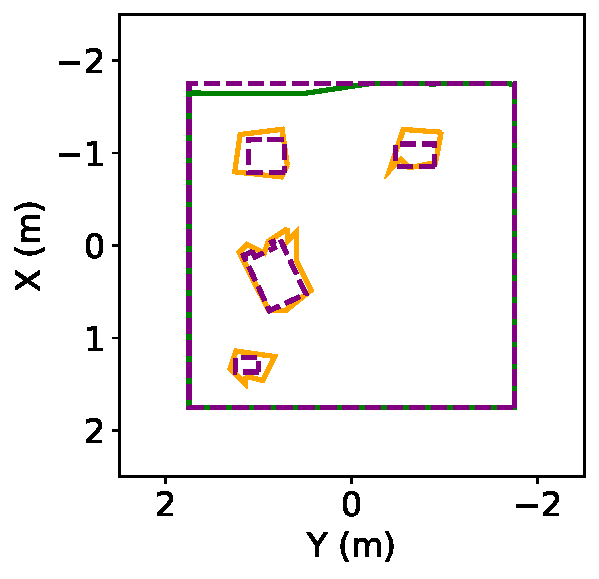
\includegraphics[clip,trim=0cm 0cm 0cm 0cm,width=.99\linewidth]{chapter_7_experiments/imgs/man_poly_1.pdf}
    \caption{\label{fig:ch7_man_poly_a}}
  \end{subfigure}
  \begin{subfigure}[t]{.33\linewidth}
    \centering  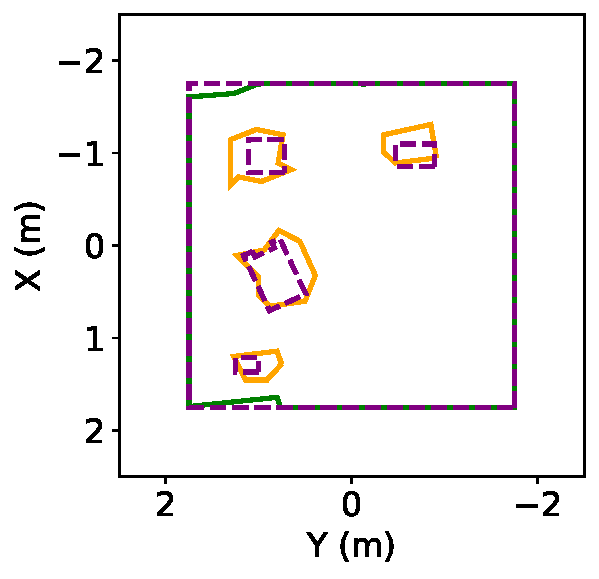
\includegraphics[clip,trim=0cm 0cm 0cm 0cm,width=.99\linewidth]{chapter_7_experiments/imgs/man_poly_3.pdf}
    \caption{\label{fig:ch7_man_poly_b}}
  \end{subfigure}
   \caption[Real-time constructed meshes and polygons during hand carry test]{Real-time constructed meshes and polygons during a hand carry test. (a,b) Meshes, polygons, and touchdown points from two hand carry tests. Polygons are in green/orange and the touchdown circle in blue. (c,d) Comparisons of the ground truth polygon (dashed purple) versus extracted polygons.} \label{fig:ch7_mesh_handcarry}
%   (\subref{fig:ch7_mesh_a}, \subref{fig:ch7_mesh_b}) 
\end{figure}


Five hand-carry tests were performed in the Flight Lab. An identical software suite as presented in Section \ref{sec:ch7_software} was running except landing commands to the quadrotor were disabled. To simulate flight, we attached an extendable pole to the sensor package.  The package was then picked up and moved around within the environment. The landing software automatically created meshes of the environment and used Polylidar3D to extract flat surfaces for landing areas.  A risk-optimal touchdown point was then selected by finding the greatest inscribed circle within the polygon. Figures~\ref{fig:ch7_mesh_a},\subref{fig:ch7_mesh_b} show qualitative results for the mesh, polygon, and touchdown point for two of the hand-carry tests. The green and orange lines represent the exterior shell of the polygon and interior holes (obstacles), respectively. The center of the blue circle denotes the risk-optimal touchdown point. 

Figures~\ref{fig:ch7_man_poly_a},\subref{fig:ch7_man_poly_b} display the same polygons shown in (a,b) but projected to the $XY$ plane alongside the ground truth workspace previously shown in Figure\ref{fig:ch7_workspace_b}. The landable area and obstacles are accurately captured in both examples. Our methods intentionally slightly exaggerate the size of obstacles to provide a safety buffer for landing.  We provide quantitative accuracy results by calculating the \ac{IOU} of each extracted polygon and the ground truth workspace polygon.  The mean \ac{IOU} for all five tests was $94.2\%$ which indicates that the surface extraction was highly accurate. There seems to be a small positional bias ($< .05m$) in obstacle placement which may be from inaccurate localization in the T265 tracking sensor. The is investigated more thoroughly in Section \ref{sec:ch7_results_t265_accuracy}.


\subsection{Flight Tests} \label{sec:ch7_results_flight}

Three flight tests were conducted with the sensor package payload. In all experiments a University of Michigan graduate student with remote piloting experience acted as \ac{PIC} and manually controlled the quadrotor to execute the flight path shown in Figure \ref{fig:ch7_flight_path}. This box pattern allowed full coverage of the workspace by the L515 LiDAR during the integration process.  A flow diagram of the experiment protocol is shown in Figure \ref{fig:ch7_flight_protocol}.  After scanning the environment, the urgent landing protocol was activated which extracted a mesh of the environment, found the optimal touchdown point, and began autonomous trajectory generation, navigation and landing procedures. In all flight tests the quadrotor successfully found the touchdown point and landed. Each flight experiment took approximately 75 seconds.


\begin{figure}[!htb]
    \centering  
    \includegraphics[page=3,width=.40\linewidth]{chapter_7_experiments/imgs/ExperimentSetup.pdf}
    \caption[Visualization of flight path used in all experiments]{Visualization of flight path used in all experiments.\label{fig:ch7_flight_path}}
\end{figure}

\begin{figure}[!htb]
    \centering  
   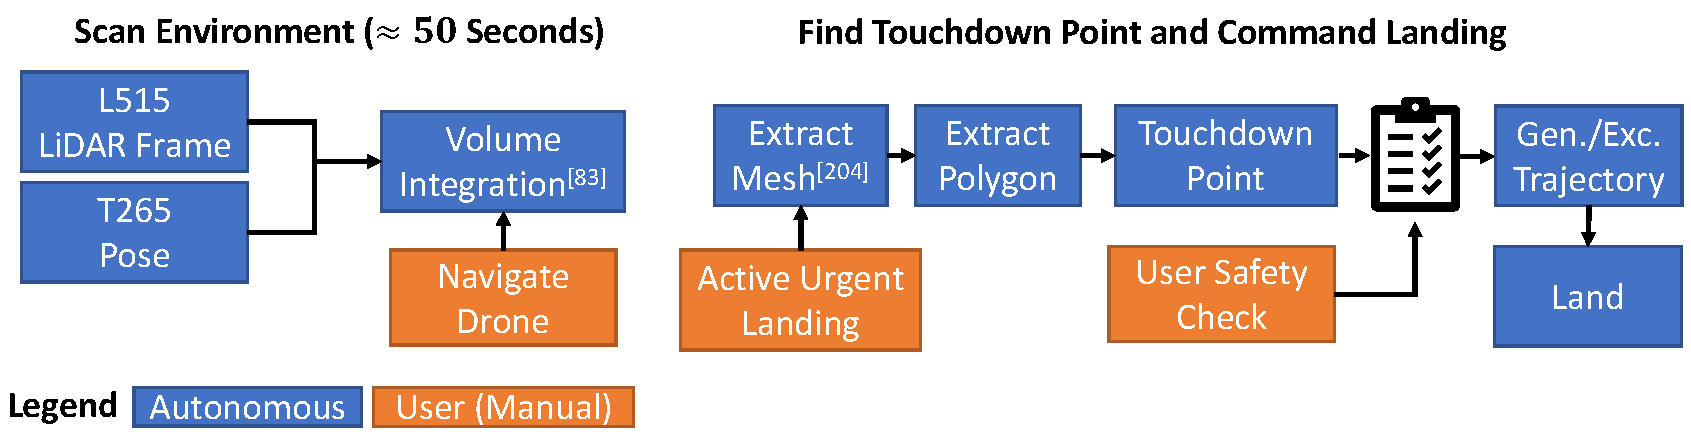
\includegraphics[width=.80\linewidth]{chapter_7_experiments/imgs/LandingProtocol.pdf}
    \caption[Flow diagram of flight experiment protocol]{Flow diagram of flight experiment protocol.\label{fig:ch7_flight_protocol}}
\end{figure}
 
% \begin{figure}[!htb]
%     \centering
%   \begin{subfigure}[t]{.25\linewidth}
%     \centering  \includegraphics[page=3,width=.99\linewidth]{chapter_7_experiments/imgs/ExperimentSetup.pdf}
%     \caption{Flight path\label{fig:ch7_flight_path}}
%   \end{subfigure}
%   \begin{subfigure}[t]{.73\linewidth}
%     \centering  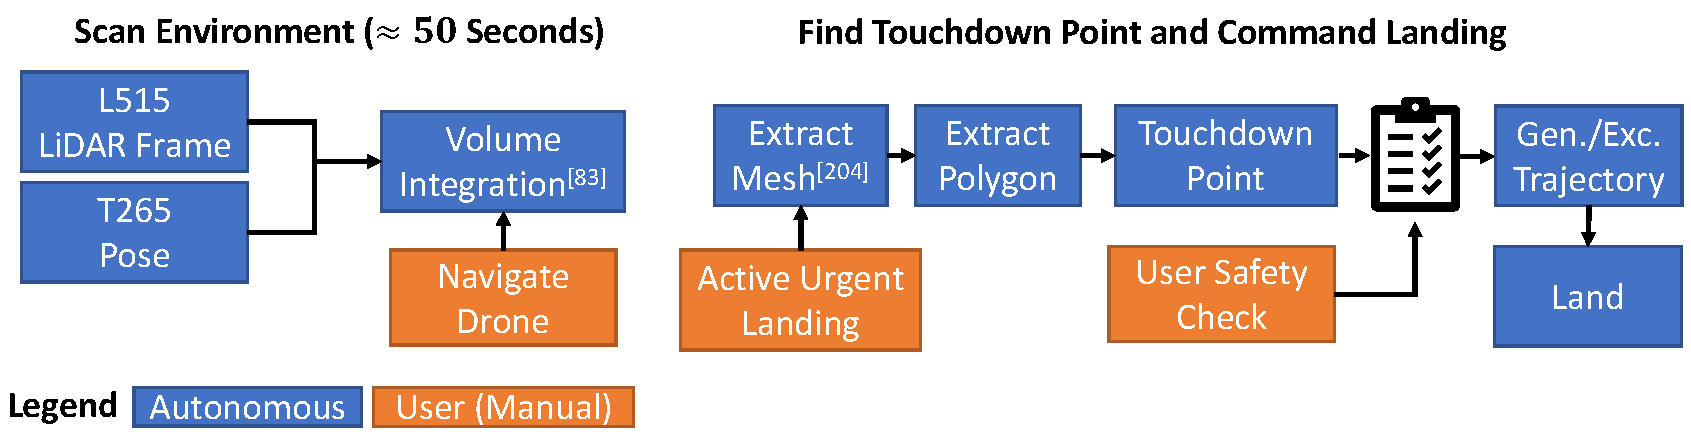
\includegraphics[width=.99\linewidth]{chapter_7_experiments/imgs/LandingProtocol.pdf}
%     \caption{Experiment protocol\label{fig:ch7_flight_protocol}}
%   \end{subfigure}
%   \caption{Flight path and experiment protocol\label{fig:ch7_flight_protocol_all}. }
% \end{figure}



Figures~\ref{fig:ch7_flight_mesh_a},\subref{fig:ch7_flight_mesh_b} show the meshes generated in real-time from the flight experiments. We can see that the mesh, polygons, and touchdown point are accurate of the environment. Figures~\ref{fig:ch7_man_poly_a},\subref{fig:ch7_man_poly_b} show the extracted polygons projected to the $XY$ plane and compared with the ground truth polygon of the workspace. The mean \ac{IOU} for all three flight tests was $92.7\%$, slightly lower than the $94.3$\% accuracy of the hand carry tests.  This may indicate that the T265 struggled with more precise localization in flight versus being hand carried. 

\begin{figure}[!htb]
  \centering
  \begin{subfigure}[t]{.29\linewidth}
    \centering  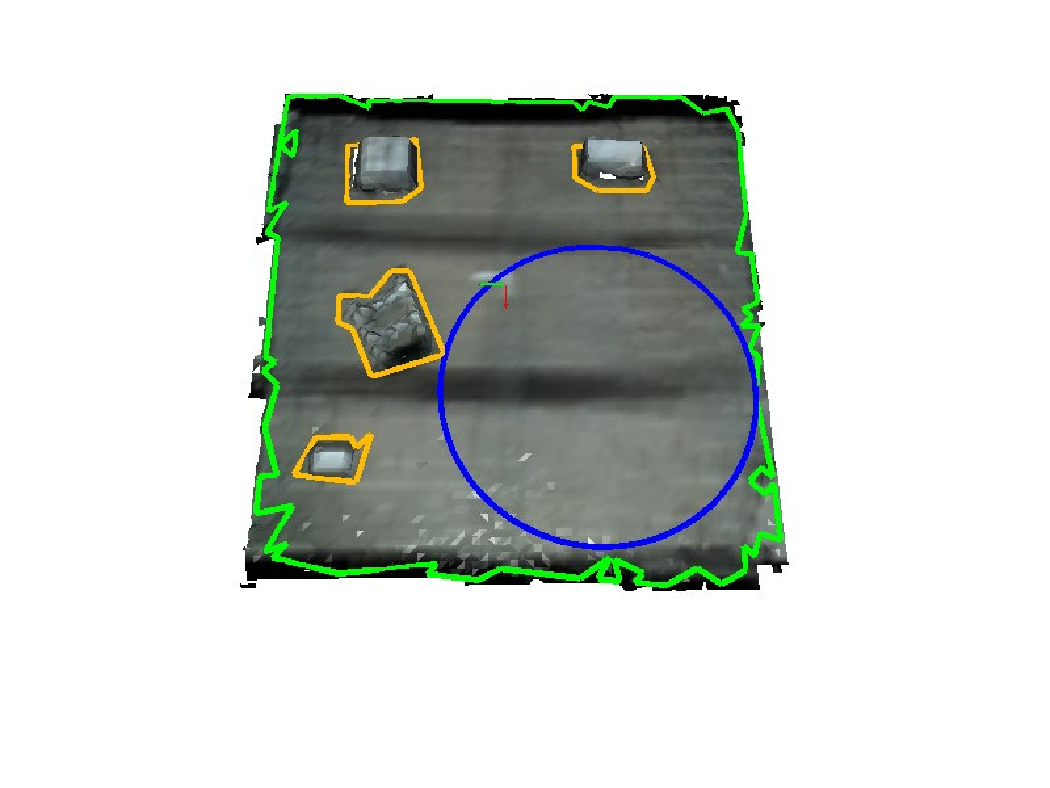
\includegraphics[page=1,clip,trim=3.5cm 3cm 3.5cm 1.0cm,width=.99\linewidth]{chapter_7_experiments/imgs/mesh_flight.pdf}
    \caption{\label{fig:ch7_flight_mesh_a}}
  \end{subfigure}
  \begin{subfigure}[t]{.29\linewidth}
    \centering  \includegraphics[page=2,clip,trim=3.5cm 3cm 3.5cm 1.0cm,width=.99\linewidth]{chapter_7_experiments/imgs/mesh_flight.pdf}
    \caption{\label{fig:ch7_flight_mesh_b}}
  \end{subfigure}
  \begin{subfigure}[t]{.29\linewidth}
    \centering  \includegraphics[page=3,clip,trim=3.5cm 3cm 3.5cm 1.0cm,width=.99\linewidth]{chapter_7_experiments/imgs/mesh_flight.pdf}
    \caption{\label{fig:ch7_flight_mesh_c}}
  \end{subfigure}
  
  \begin{subfigure}[t]{.32\linewidth}
    \centering  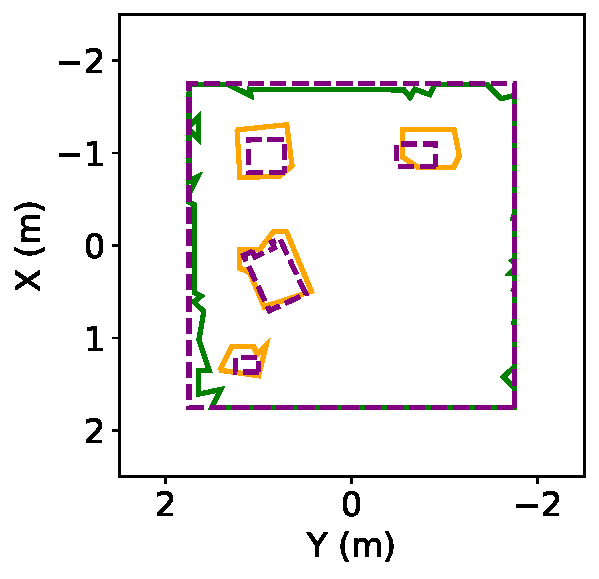
\includegraphics[clip,trim=0cm 0cm 0cm 0cm,width=.99\linewidth]{chapter_7_experiments/imgs/flight_poly_1.pdf}
    \caption{\label{fig:ch7_flight_poly_a}}
  \end{subfigure}
  \begin{subfigure}[t]{.32\linewidth}
    \centering  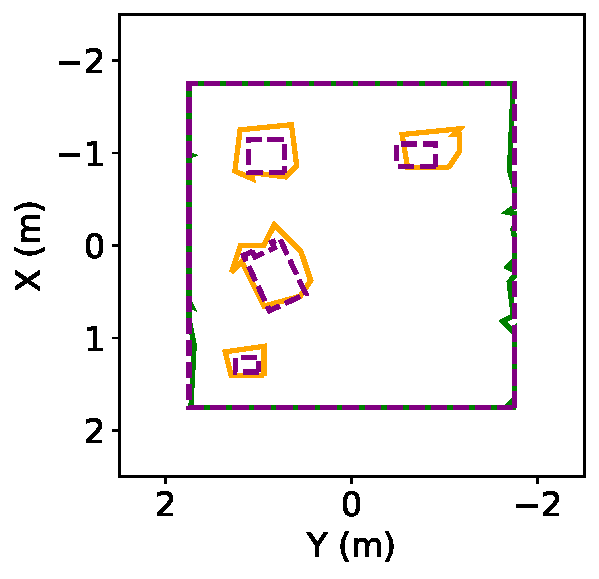
\includegraphics[clip,trim=0cm 0cm 0cm 0cm,width=.99\linewidth]{chapter_7_experiments/imgs/flight_poly_2.pdf}
    \caption{\label{fig:ch7_flight_poly_b}}
  \end{subfigure}
  \begin{subfigure}[t]{.32\linewidth}
    \centering  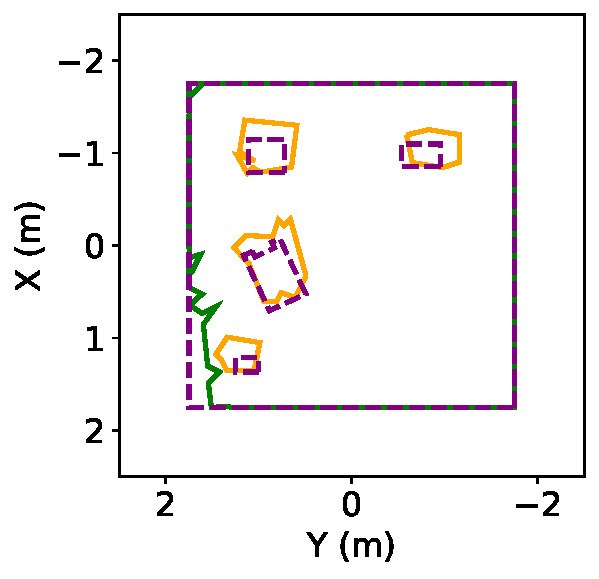
\includegraphics[clip,trim=0cm 0cm 0cm 0cm,width=.99\linewidth]{chapter_7_experiments/imgs/flight_poly_3.pdf}
    \caption{\label{fig:ch7_flight_poly_c}}
  \end{subfigure}
  \caption[Real-time constructed meshes and polygons during flight test]{Real-time constructed meshes and polygons during flight test. (a,b,c) Meshes, polygons, and touchdown points from three flight tests, respectively. The polygon is shown in green/orange and touchdown circle in blue. (c,d,e) Comparisons of the ground truth polygon (purple) versus extracted polygons. }\label{fig:ch7_mesh_flight}
%   (\subref{fig:ch7_mesh_a}, \subref{fig:ch7_mesh_b}) 
\end{figure}


\subsection{Execution Time} \label{sec:ch7_results_execution_time}

The computation time for the major steps in our methods are calculated and presented in Table \ref{table:ch7_execution_time}. The table shows the mean execution time and standard deviation for all experiments conducted on both the low-power Odyssey x86 \ac{SBC} as well as a desktop computer. Both computers ran the same software over recorded data for all experiments. The Odyssey board has an Intel J4105 processor with 4 Cores and 8 GB of RAM while the desktop is configured with a 12 core AMD 3900X processor with 32 GB of RAM. In both systems a maximum of 2 threads were used for parallelization in Polylidar3D for polygon extraction. All other steps are single threaded. 

For each test approximately 111 \ac{RGBD} frames were integrated into a voxel volume.  Once the volume is created, a triangular mesh of the environment is extracted.  Polylidar3D then extracts a polygon of the mesh, filters/simplifies it, and an optimal touchdown point is found. The Odyssey \ac{SBC} executes volume integration sufficiently fast to match the real-time 6 Hz stream of the LiDAR sensor. Additionally, our landing site selection software is able to find a safe landing site in less than 60 ms. In most cases the desktop computer is $\approx3$ times faster than the Odyssey \ac{SBC}. However, frame integration has a 10X performance degradation when using the Odyssey board in comparison to the desktop computer.  This can be seen not only from the average execution times but also the large standard deviation of 27ms. 

\begin{table}[H]
\centering
\caption{Mean and standard deviation of execution times (ms)}\label{table:ch7_execution_time}
\resizebox{\columnwidth}{!}{
\begin{tabular}{c@{\qquad}cc@{\qquad}ccc}
  \toprule 
  \multirow{2}{*}{\raisebox{-\heavyrulewidth}{\textbf{Computer}}} & \multicolumn{2}{c}{\textbf{Volume Integration}} & \multicolumn{3}{c}{\textbf{Touchdown Point Selection}} \\
  \cmidrule{2-6}
   &  \textbf{Integrate Frame} & \textbf{Extract Mesh} & \textbf{Extract Polygon} & \textbf{Filter Polygon} & \textbf{Touchdown Point} \\
  \midrule 
  Odyssey \ac{SBC} & $19.6 \pm 27.2 $ & $47.8 \pm 8.4$ & $18.3 \pm 2.9$ & $39.1 \pm 9.2$ & 0.2  \\
  Desktop     & $2.5 \pm 0.5$  & $16.9 \pm 2.6$ & $6.7 \pm 0.9$  & $14.0 \pm 5.1$ &  $0.1$  \\
  \bottomrule
\end{tabular}
}
\end{table}


\subsection{Trajectory Error Analysis of Intel RealSense T265}\label{sec:ch7_results_t265_accuracy}

% The Intel RealSense T265 utilizes an unknown closed source visual odometry algorithm with loop closure. A primary benefit is that the camera itself contains an on-board ASIC to perform all SLAM calculations to output the 6DOF pose. This reduces the computational burden for flight controllers or other companion boards. The product was released in 2020 with recent papers investigating its tracking performance \cite{ouerghi:hal-02567816, 10.1007/978-3-030-70740-8_14}. However, to the authors knowledge no accuracy results have been reported when mounted on \ac{sUAS} with motion capture for ground truth estimates.

This section provides a trajectory error analysis of the T265 pose predictions in comparison to the ground truth \ac{MCS}. The T265 predicted pose estimates are given an initial alignment to the ground truth trajectory following standard evaluation procedures in \cite{zhang_tutorial_2018}. Figure \ref{fig:ch7_flight_path_3d} shows the 3D trajectory of the quadrotor in the first flight experiment using pose estimates from the \ac{MCS} (orange) and the T265 (blue). The predicted T265 trajectory closely follows \ac{MCS} but appears to drift away marginally after time. Figure \ref{fig:ch7_t265} provides time response plots for the $x, y, z$, roll, pitch, and yaw estimates for all three flight experiments.

\begin{figure}[!ht]
    \centering  
    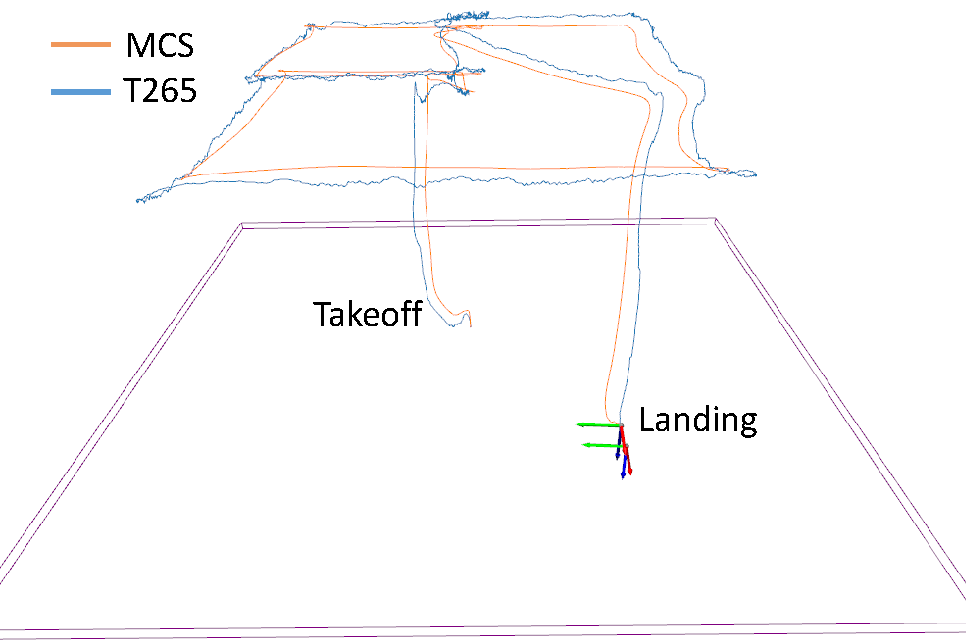
\includegraphics[page=1,clip,trim=0cm 0cm 0cm 0cm,width=.45\linewidth]{chapter_7_experiments/imgs/flight_path_t265_mcs.pdf}
    \caption[Trajectory of quadrotor from flight \#1 ]{Trajectory of quadrotor from Flight \#1. Trajectory of Motion Capture System (orange) and T265 (blue) shown. }\label{fig:ch7_flight_path_3d}
\end{figure}

\begin{figure}[!ht]
  \centering
  \begin{subfigure}[t]{.90\linewidth}
    \centering  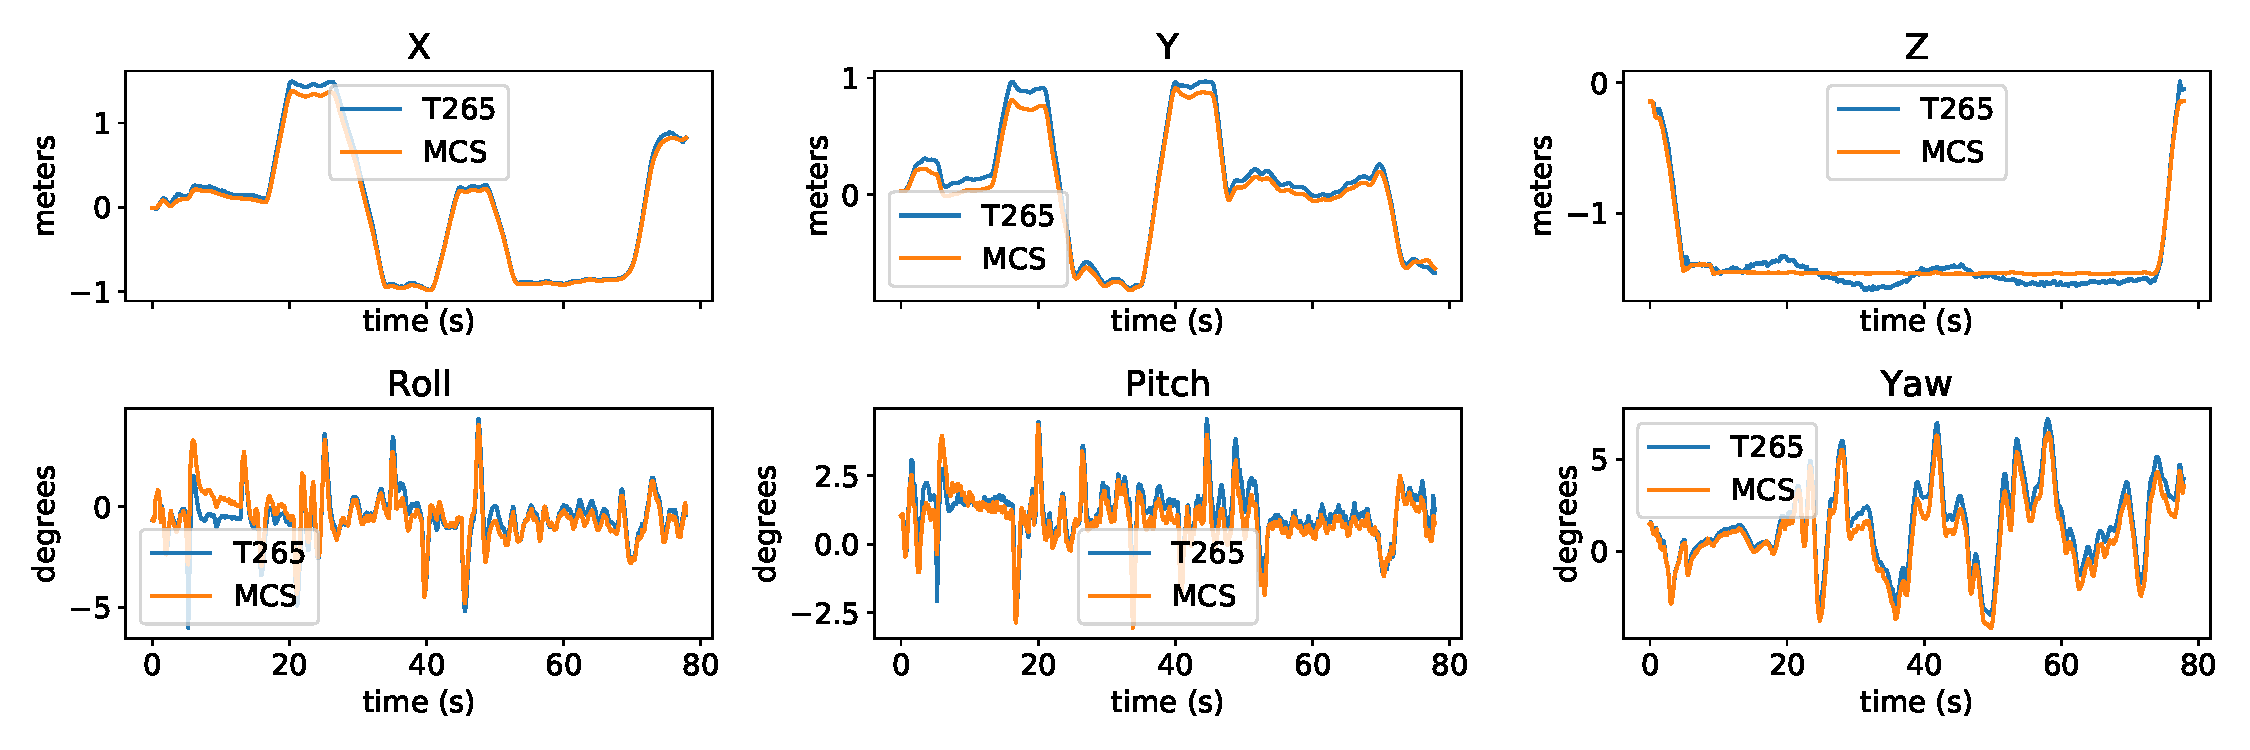
\includegraphics[width=.99\linewidth]{chapter_7_experiments/imgs/t265_gt_graphs_flight_1.pdf}
    \caption{\label{fig:ch7_t265_a}Flight \#1}
  \end{subfigure}
  \begin{subfigure}[t]{.90\linewidth}
    \centering  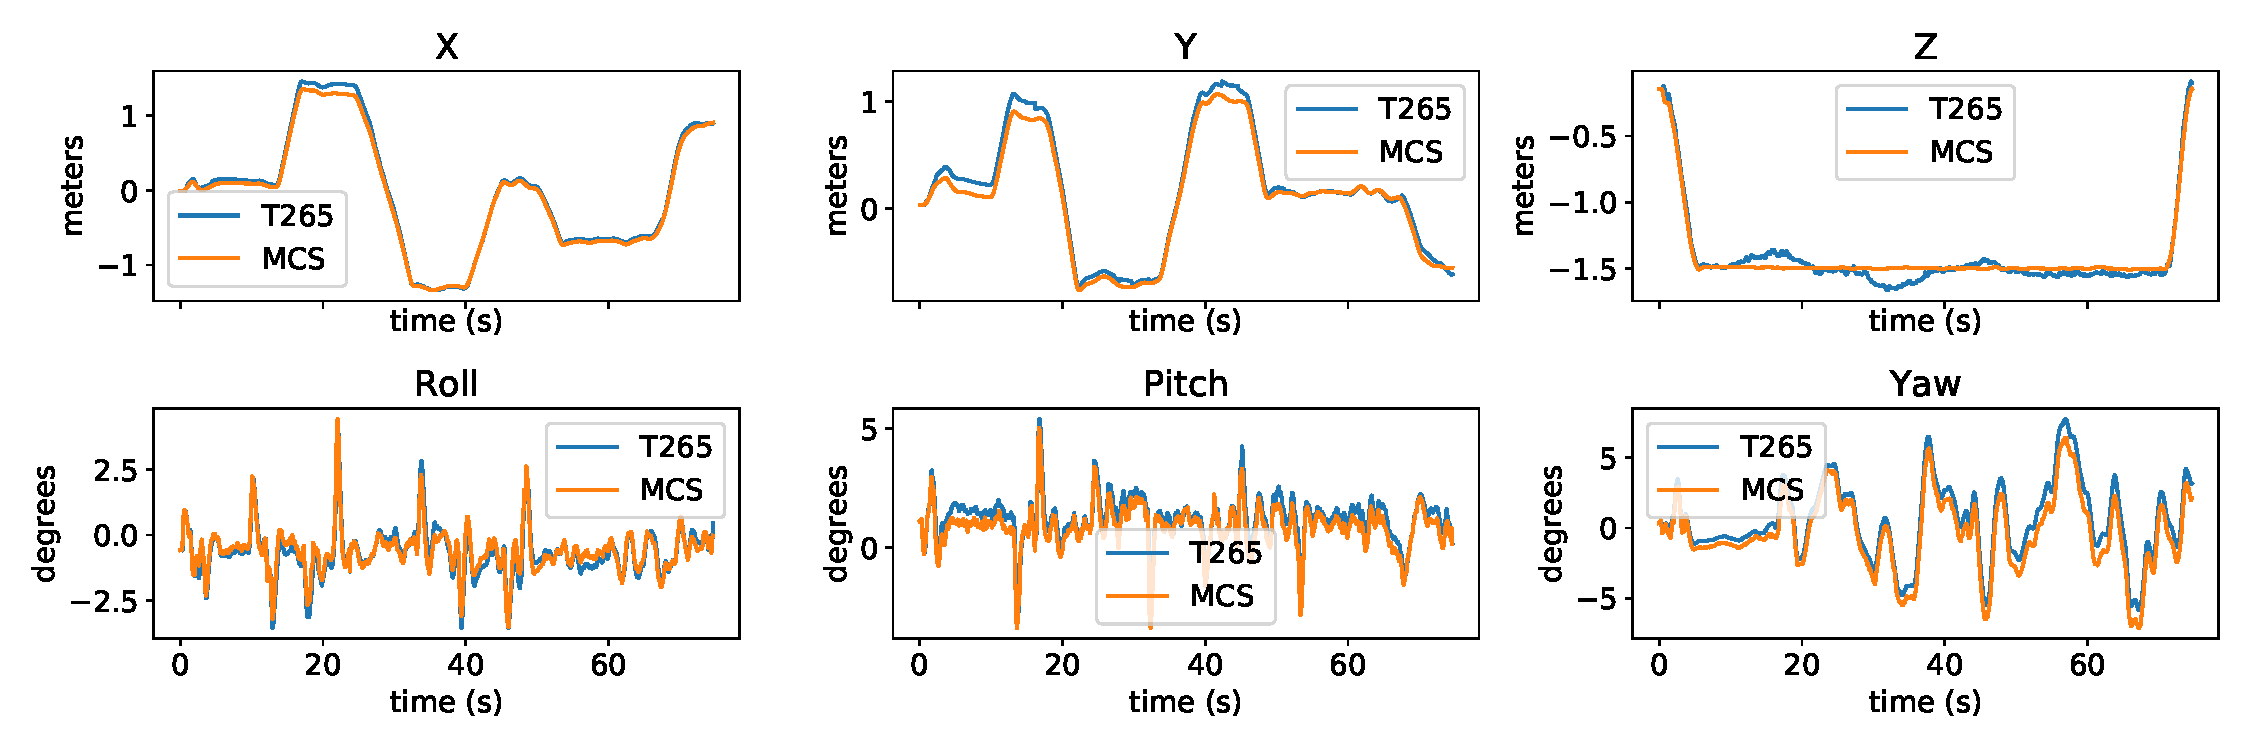
\includegraphics[width=.99\linewidth]{chapter_7_experiments/imgs/t265_gt_graphs_flight_2.pdf}
    \caption{\label{fig:ch7_t265_b}Flight \#2}
  \end{subfigure}
  \begin{subfigure}[t]{.90\linewidth}
    \centering  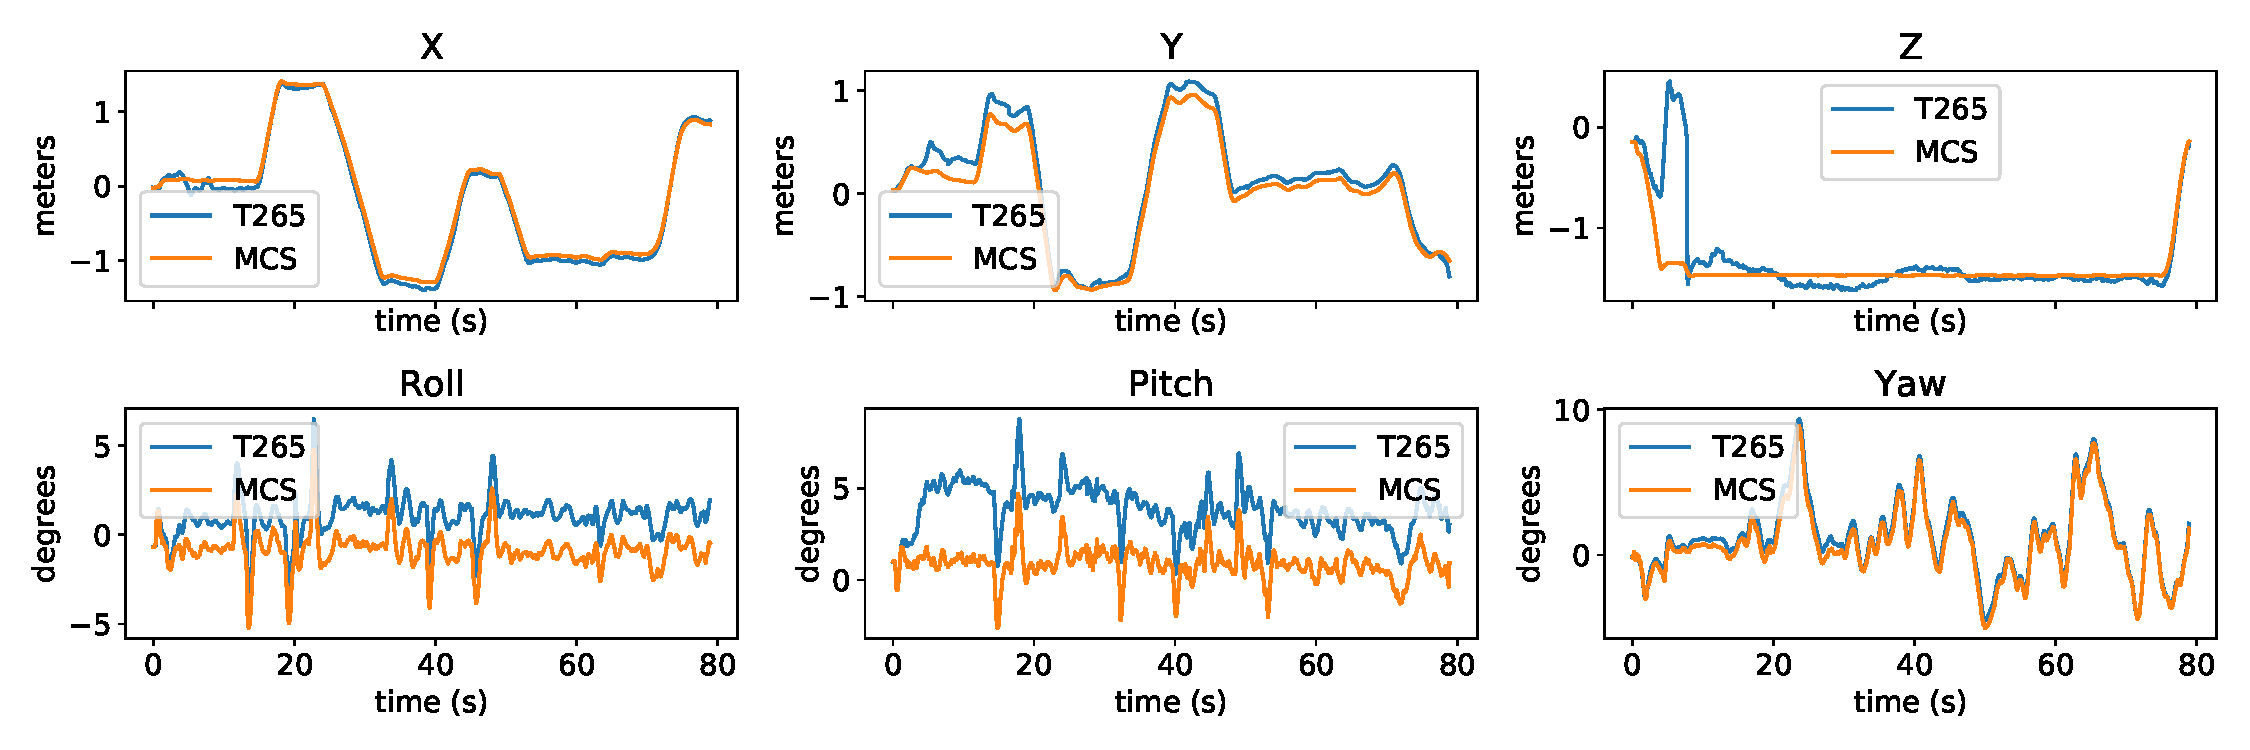
\includegraphics[width=.99\linewidth]{chapter_7_experiments/imgs/t265_gt_graphs_flight_3.pdf}
    \caption{\label{fig:ch7_t265_c}Flight \#3}
  \end{subfigure}
  \caption[Comparison of Motion Capture System (MCS) versus T265]{Comparison of Motion Capture System (MCS) versus T265.}\label{fig:ch7_t265}
\end{figure}
The mean absolute trajectory error is calculated for each flight and displayed in Table \ref{table:ch7_ate}. The position and rotation error are computed following procedures in \cite{zhang_tutorial_2018}. The average length of each flight experiment path is approximately 17.2m. The position and rotation error is low for the first and second flight but markedly higher in the third flight. During take-off of the third flight the T265 had strong deviations in altitude, roll, and pitch from the \ac{MCS} as seen in Figure \ref{fig:ch7_t265_c}. The estimated roll and pitch continued to track correctly but with a large bias of approximately 4 degrees.  The positional altitude quickly recovered after 5 seconds when the T265 experienced a ``pose jump'' after a loop closure occurred. Currently ``pose jumping'' for the T265 is only implemented for translation and does not correct orientation error \cite{realsense_github_t265}.

\begin{table}[h]
\centering
\caption{Mean Absolute Trajectory Error (ATE) for T265}\label{table:ch7_ate}
\begin{tabular}{@{}lccc@{}}
\toprule
Trial    & Length (m) & Mean $\textrm{ATE}_{\textrm{pos}}$ (m) & Mean $\textrm{ATE}_{\textrm{rot}}$ (deg) \\ \midrule
Flight \#1 & 17.1       & 0.11                  & 0.98                    \\
Flight \#2 & 16.6       & 0.10                  & 1.03                    \\
Flight \#3 & 17.9       & 0.35                  & 3.7                     \\ \bottomrule
\end{tabular}
\end{table}


\section{Conclusion and Future Work}

Multiple experiments were conducted to validate our proposed methods for real-time touchdown point selection. We developed a sensor package that holds an Intel RealSense L515 LiDAR, RealSense T265 Tracking Camera, and an Odyssey x86 \acf{SBC}. Together they provide depth data, localization and mapping, and the computational power necessary for our landing software. The sensor package was both hand-carried and flown with a quadrotor in an obstacle cluttered indoor environment. Accurate meshes of the environment were generated in real-time for which landing sites were extracted as polygons. The polygons representing safe landing areas were compared against the ground truth map and found to be accurate. In every experiment a safe landing zone was found which correctly minimized risk. 

Future work should be performed to expand upon the diversity and placement of obstacles in the workspace.  For example, adding larger more non-convex obstacles with holes in the center will further challenge our methods to more fully verify their efficacy. In addition, highly cluttered environments should be tested to verify our touchdown point selection algorithm will only select safe landing points. The size of the environment, the number of obstacles, and obstacle shape complexity will have an impact on the computation time needed for our landing software. Further work should be performed to quantify this relationship and determine its impact.  Experimental work should also be conducted to integrate a semantic neural network with Polylidar3D as proposed in Chapter \ref{ch:landingsim}. Data of real-world and synthetic environments should be captured and labelled to train the proposed network. The Odyssey board should be swapped with a \ac{SBC} with an on-board \ac{GPU} to provide minimal inference time for semantic segmentation. Further flight experiments above real-world city rooftops can then be conducted to further validate our touchdown point selection algorithm.